\section{Controlling the electron number}
\label{sec:electron-number-control}

To use confined electrons as spin qubits, we must prepare the charge
configuration assumed by the spin model and retain it during control.
The single-spin qubit considered below requires one electron in a dot;
our two-dot spin model starts with one electron in each dot. A reservoir
supplies these electrons through tunneling. Gate voltages change the
dot energies to select the desired occupations, while the barriers
control how readily electrons can enter or leave. Preparing a useful
spin system therefore requires control of both its energetically
preferred electron number and its exchange of electrons with the reservoir.

To compare different electron numbers, we account for the energy of
both the dot and the reservoir that supplies its electrons. Adding
an electron to an $(N-1)$-electron dot costs $E_N-E_{N-1}$.
At zero temperature, the large reservoir loses one electron, changing
its energy by $-\mu_{\mathrm R}$, where $\mu_{\mathrm R}$ is its chemical potential.
The transfer lowers the combined energy when
$E_N-E_{N-1}-\mu_{\mathrm R}<0$. For $N$ electrons transferred
from the reservoir into the dot, the corresponding energy to compare
is $E_N-\mu_{\mathrm R}N$, up to a common reservoir reference.

We collect these charge sectors in the full dot Hamiltonian $H$,
which acts as $H_N$ in each $N$-electron sector.
At zero temperature, a dot in equilibrium with a weakly coupled
reservoir of chemical potential $\mu_{\mathrm R}$ occupies a
ground state of
\begin{equation}
  \widehat{\Omega}=H-\mu_{\mathrm R}\widehat N,
  \label{eq:dot-grand-canonical-hamiltonian}
\end{equation}
where $\widehat N$ counts electrons. In the $N$-electron sector,
this operator is $H_N-\mu_{\mathrm R}N$, whose ground-state
energy is $E_N-\mu_{\mathrm R}N$.
The equilibrium electron number is therefore
\begin{equation}
  \boxed{
  N_{\mathrm{eq}}(\mu_{\mathrm R})
    \in\operatorname*{arg\,min}_{N=0,1,\ldots}
                         [E_N-\mu_{\mathrm R}N]}.
  \label{eq:dot-equilibrium-electron-number}
\end{equation}
This determines the relation between chemical potential and
electron number from the energies $E_N$, at fixed dot parameters~\cite{Beenakker1991}.

\paragraph{Addition thresholds and charge gaps.}
Equating $E_N-\mu_{\mathrm R}N$ and
$E_{N-1}-\mu_{\mathrm R}(N-1)$ gives the threshold for adding
the $N$th electron:
\begin{equation}
  \mu_N=E_N-E_{N-1}.
  \label{eq:dot-addition-threshold}
\end{equation}
The spacing between successive thresholds is
\begin{equation}
  E_{\mathrm{add}}(N)=\mu_{N+1}-\mu_N
       =E_{N+1}-2E_N+E_{N-1}.
  \label{eq:dot-addition-energy-spacing}
\end{equation}
If $E_N$ is strictly convex, meaning $E_{\mathrm{add}}(N)>0$
for every $N\geq1$, these thresholds increase in order.
Minimizing $E_N-\mu_{\mathrm R}N$ then selects charge $N\geq1$
throughout the interval
\begin{equation}
  \mu_N<\mu_{\mathrm R}<\mu_{N+1}.
  \label{eq:dot-charge-stability-window}
\end{equation}
Each plateau has width $E_{\mathrm{add}}(N)$, so electrons enter
one at a time as $\mu_{\mathrm R}$ increases. At a boundary,
neighboring charges are degenerate; the empty dot is selected
for $\mu_{\mathrm R}<\mu_1$. Without strict convexity, some
plateaus can disappear, and the original minimization remains
the general rule.

Within a plateau, adding or removing one electron changes
the energy of $\widehat{\Omega}$ by
\begin{align}
  \Delta_+&=E_{N+1}-E_N-\mu_{\mathrm R}
             =\mu_{N+1}-\mu_{\mathrm R},\\
  \Delta_-&=E_{N-1}-E_N+\mu_{\mathrm R}
             =\mu_{\mathrm R}-\mu_N.
  \label{eq:dot-charge-transfer-costs}
\end{align}
Both costs are positive, suppressing low-energy sequential
charge transfer: this is the Coulomb-blockade regime~\cite{Beenakker1991}.

\paragraph{Selecting a charge state with gate voltages.}
Gate voltages control the electron number through their effect on
the electric potential $\Phi(\mathbf r)$ in the dot. For an electron
of charge $-e$, a potential change $\delta\Phi(\mathbf r)$ gives a
potential energy shift $-e\,\delta\Phi(\mathbf r)$. This alters the many-electron energies
$E_N$ and the addition thresholds $\mu_N=E_N-E_{N-1}$.
For a uniform shift $\delta\Phi$ over the dot,
$\delta E_N=-Ne\,\delta\Phi$, so $\delta\mu_N=-e\,\delta\Phi$.
With the reservoir chemical potential $\mu_{\mathrm R}$ held fixed,
moving a threshold across it changes the equilibrium electron
number according to Eq.~\eqref{eq:dot-equilibrium-electron-number}.
Electrical transport or charge sensing can detect this change
(Appendix~\ref{app:charge-detection}). For a given gate geometry,
a first-order expansion about a reference voltage setting
$\mathbf V_0$ relates the threshold shift to the applied voltage changes:
\begin{equation}
 \delta\mu_N\simeq-e\sum_g\alpha_{Ng}\,\delta V_g,
 \qquad
 \alpha_{Ng}=-\frac1e
       \left.\frac{\partial\mu_N}{\partial V_g}\right|_{\mathbf V_0}.
 \label{eq:platform-gate-response}
\end{equation}
Here $\alpha_{Ng}$ is the dimensionless \emph{lever arm} of gate $g$
for the $N$th addition threshold: $e\alpha_{Ng}$ converts a change
in gate voltage into a shift of that threshold. A physical gate
generally alters both the dot levels and the tunneling barriers,
so both effects must be considered when choosing the operating
voltages. Appendix~\ref{app:voltage-response} derives the corresponding
voltage responses.

\subsection{Loading a single dot}
\label{sec:single-dot-loading}

For the single-spin qubit, the two logical states are spin states
of the same confined electron. The required charge state is therefore
$N=1$. \emph{Loading} prepares this occupation by bringing an electron
from the reservoir into the dot through tunneling.

Figure~\ref{fig:single-dot-loading} shows the charge regions along
a gate-voltage scan at fixed $\mu_{\mathrm R}$. To prepare $N=1$,
first empty the dot at a setting such as $E$:
set $\mu_1-\mu_{\mathrm R}\gg k_BT$ while allowing tunneling to the reservoir,
so that an electron already in the dot can escape. Then change the
gate voltage to a setting such as $L$, where
$\mu_1<\mu_{\mathrm R}<\mu_2$, keeping the reservoir barrier low
enough to permit tunneling. An electron from an occupied reservoir
state can now enter the dot. Once it has entered, adding a second
electron costs $\mu_2-\mu_{\mathrm R}>0$, and removing the first
costs $\mu_{\mathrm R}-\mu_1>0$. Choosing both costs large compared
with $k_BT$ suppresses these further charge changes and selects
single occupation.

\begin{figure}[htbp]
 \centering
 % Single-dot charge regions as a function of gate voltage.
% Increasing V_g lowers the addition energies (positive lever arm).
% E and L denote the empty and loading operating points; the arrow is
% only the gate-voltage pulse, not a change in the tunnel barrier.
\begingroup
\definecolor{loadingGate}{HTML}{0072B2}
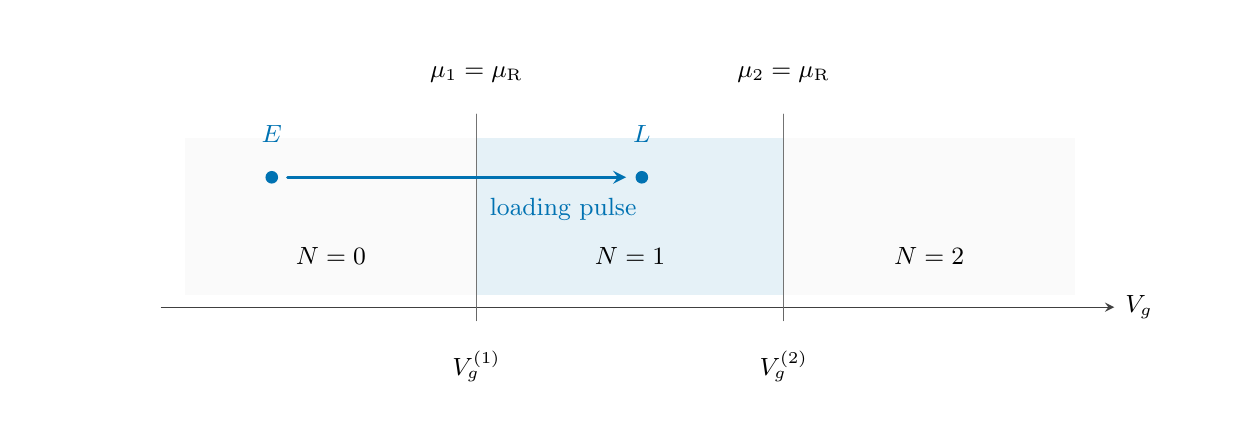
\begin{tikzpicture}[
 x=1mm,y=1mm,>=stealth,line cap=round,line join=round,
 every node/.style={font=\small,inner sep=1pt}
]
 \path[use as bounding box] (0,3) rectangle (150,52);

 % Charge sectors at a fixed reservoir chemical potential.
 \fill[black!2] (20,18) rectangle (133,38);
 \fill[loadingGate!10] (57,18) rectangle (96,38);
 \draw[black!55,line width=0.5pt] (57,16.5)--(57,41);
 \draw[black!55,line width=0.5pt] (96,16.5)--(96,41);
 \node at (38.5,23) {$N=0$};
 \node at (76.5,23) {$N=1$};
 \node at (114.5,23) {$N=2$};
 \node at (57,46) {$\mu_1=\mu_{\mathrm R}$};
 \node at (96,46) {$\mu_2=\mu_{\mathrm R}$};

 % A pulse crosses the first threshold and stops inside the N=1 interval.
 \fill[loadingGate] (31,33) circle (0.8);
 \fill[loadingGate] (78,33) circle (0.8);
 \draw[->,loadingGate,line width=1.05pt] (33,33)--(76,33);
 \node[text=loadingGate] at (31,38.5) {$E$};
 \node[text=loadingGate] at (78,38.5) {$L$};
 \node[text=loadingGate,fill=loadingGate!10,inner sep=0.5pt]
      at (68,29) {loading pulse};

 % Gate axis and charge-degeneracy voltages.
 \draw[->,black!75,line width=0.5pt] (17,16.5)--(138,16.5);
 \node[anchor=west] at (139,16.5) {$V_g$};
 \foreach \tickX in {57,96}{
  \draw[black!60,line width=0.4pt]
       (\tickX,16.5)--(\tickX,14.8);
 }
 \node at (57,9) {$V_g^{(1)}$};
 \node at (96,9) {$V_g^{(2)}$};
\end{tikzpicture}
\endgroup

 \caption{Single-dot charge regions at fixed reservoir chemical
 potential $\mu_{\mathrm R}$. For the gate response illustrated here,
 increasing $V_g$ lowers the addition thresholds. The voltages
 $V_g^{(1)}$ and $V_g^{(2)}$ satisfy $\mu_1=\mu_{\mathrm R}$ and
 $\mu_2=\mu_{\mathrm R}$, respectively. The loading pulse moves from
 the empty-dot setting $E$ into the $N=1$ region at $L$, while
 tunneling to the reservoir remains possible. Raising the reservoir
 barrier after loading is a separate step.}
 \label{fig:single-dot-loading}
\end{figure}

Crossing the addition threshold makes entry energetically favorable;
the dot still has to wait for an electron to tunnel through the
barrier. The loading voltages are therefore held for a finite
interval, long compared with the typical entry waiting time, which
depends on the barrier transparency. After this loading interval,
raising the reservoir barrier reduces electron exchange and retains
the electron while its spin is manipulated. For an unwanted escape
rate $\Gamma_{\mathrm{escape}}$ and a control interval $\tau$, the
condition $\Gamma_{\mathrm{escape}}\tau\ll1$ makes loss during that
interval unlikely. Energetic stability suppresses unwanted charge
changes through their energy costs; a high barrier additionally
suppresses the tunneling that would carry them out.

\FloatBarrier
\subsection{Loading two coupled dots}
\label{sec:double-dot-loading}

The two-dot spin model used below requires one localized spin on
each dot. Its starting charge configuration is therefore $(N_1,N_2)=(1,1)$.
Preparing it requires selecting the occupation of each dot, since
two electrons in the pair could also occupy $(2,0)$ or $(0,2)$.

The plunger-gate voltages $V_1,V_2$ tune the dot energies. Repulsion
between dots makes each addition threshold depend on the occupation
of the other dot. With the reservoirs at a common chemical potential
$\mu_{\mathrm R}$ and interdot mixing neglected, the equilibrium
condition partitions the $(V_1,V_2)$ plane into regions of fixed
$(N_1,N_2)$ (Appendix~\ref{app:charge-stability}).
Figure~\ref{fig:measurement-honeycomb} shows the resulting
\emph{charge stability diagram} around $(1,1)$. Crossing a blue
boundary exchanges an electron with a reservoir; for example,
$(1,0)\to(1,1)$ loads dot 2. Crossing an orange boundary transfers
an electron between dots while preserving their total number;
for example, $(1,1)\to(2,0)$ moves an electron from dot 2 to dot 1.

\begin{figure}[htbp]
 \centering
 % A local honeycomb neighborhood with the usual negatively sloping
% reservoir transitions and positively sloping interdot transitions.
\begingroup
\small
\setlength{\unitlength}{1mm}
\begin{picture}(150,87)
 \put(15,8){\vector(1,0){122}}
 \put(15,8){\vector(0,1){73}}
 \put(137,4){\makebox(10,7){$V_1$}}
 \put(5,78){\makebox(10,7){$V_2$}}
 \put(66,35){\makebox(25,8){$(1,1)$}}
 \put(32,26){\makebox(25,8){$(0,1)$}}
 \put(53,11){\makebox(25,8){$(1,0)$}}
 \put(90,18){\makebox(25,8){$(2,0)$}}
 \put(106,44){\makebox(25,8){$(2,1)$}}
 \put(83,62){\makebox(25,8){$(1,2)$}}
 \put(28,62){\makebox(25,8){$(0,2)$}}
 \linethickness{0.9pt}
 \color{blue!65!black}
 % Central cell A(51,29), B(83,21), C(103,37),
 % D(95,61), E(63,69), F(43,53).
 \qbezier(51,29)(67,25)(83,21)
 \qbezier(103,37)(99,49)(95,61)
 \qbezier(95,61)(79,65)(63,69)
 \qbezier(43,53)(47,41)(51,29)
 % Reservoir-transition edges extending to adjacent cells.
 \qbezier(83,21)(85,15)(87,9)
 \qbezier(103,37)(118,33.25)(133,29.5)
 \qbezier(63,69)(61,75)(59,81)
 \qbezier(43,53)(31.5,55.875)(20,58.75)
 \color{orange!85!black}
 \qbezier(83,21)(93,29)(103,37)
 \qbezier(63,69)(53,61)(43,53)
 \qbezier(51,29)(40,20.2)(29,11.4)
 \qbezier(95,61)(107,70.6)(119,80.2)
 \color{black}
 \put(51,29){\circle*{2}}
 \put(83,21){\circle*{2}}
 \put(103,37){\circle*{2}}
 \put(95,61){\circle*{2}}
 \put(63,69){\circle*{2}}
 \put(43,53){\circle*{2}}
\end{picture}
\endgroup

 \caption{Schematic charge regions of two dots with negligible
 interdot mixing and a common reservoir chemical potential.
 Blue boundaries change the total electron number by one;
 orange boundaries transfer an electron between dots.
 Black points, called triple points, mark where three charge regions
 meet. The central $(1,1)$ region provides the charge configuration
 for one localized spin on each dot. The axes are plunger voltages;
 offsets, scales, and cross-couplings are unspecified.}
 \label{fig:measurement-honeycomb}
\end{figure}

To prepare $(1,1)$, choose voltages inside its region, sufficiently
far from the boundaries that unwanted charge changes cost much more
than $k_BT$. Allow exchange with the reservoirs long enough for the
occupations to equilibrate, then raise the reservoir barriers to
retain the two electrons. The interdot tunnel coupling must also
remain small compared with the relevant charge-transfer gaps to
keep the occupations close to one electron per dot. Appendix~\ref{app:charge-stability}
derives the boundary conditions and explains how measured charge
transitions locate these regions.

